\chapter{State Machines}

\def\movesto{\mathrel{\longrightarrow}}

\def\lexle{\mathrel{\preceq_{\text{lex}}}}
\def\lex<{\mathrel{\prec_{\text{lex}}}}
\def\coordle{\mathrel{\preceq_{\text{c}}}}
\def\coord<{\mathrel{\prec_{\text{c}}}}

\providecommand{\boys}{\text{the-Boys}}
\providecommand{\girls}{\text{the-Girls}}
\providecommand{\qst}{\text{$q_0$}}
\providecommand{\none}{\texttt{none}}
\providecommand{\girln}{\text{$\girls \union \set{\none}$}}
\providecommand{\boyn}{\text{$\boys \union \set{\none}$}}
\providecommand{\sere}{\text{\emph{serenading}}}
\providecommand{\suit}{\text{\emph{suitors}}}
\providecommand{\fav}{\text{\emph{favorite}}}
\providecommand{\nex}{\text{\emph{next}}}
\providecommand{\tgn}{\text{\emph{total-girls-names}}}

\hyperdef{state}{machines}{\section{State machines}}

State machines are an abstract model of step-by-step processes, and
accordingly, they come up in many areas of Computer Science.  You may
already have seen them in a digital logic course, a compiler course, or a
probability course.

\subsection{Basic definitions}

A state machine is really nothing more than a binary relation on a set,
except that the elements of the set are called ``states'' and a pair
$(p,q)$ in the graph of the relation is called a ``transition.''  The
transition from state $p$ to state $q$ will be written $p \movesto q$.
A state machine also comes equipped with a designated \emph{start state}.

State machines used in digital logic and compilers usually have only a
finite number of states, but machines that model continuing computations
typically have an infinite number of states.  In many applications, the
states, and/or the transitions have labels indicating input or output
values, costs, capacities, or probabilities, but for our purposes,
unlabelled states and transitions are all we need.\footnote{We do name
states, as in Figure~\ref{fig:counter}, so we can talk about them, but the
names aren't part of the state machine.}

\begin{example}
A bounded counter, which counts from $0$ to $99$ and overflows at 100.
The transitions are pictured in Figure~\ref{fig:counter}, with start state
zero.

\begin{figure}[htbp]
\centering 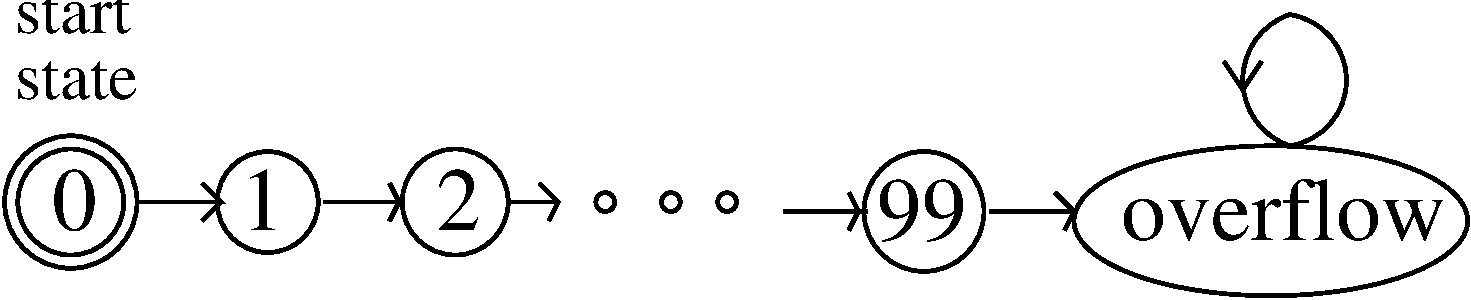
\includegraphics[height=1in]{figures/counter}
%\centerline{\psfig{figure=figures/counter.eps,height=1in}}
\caption{\em State transitions for the 99-bounded counter.}
\label{fig:counter}
\end{figure}

This machine isn't much use once it overflows, since it has no way to get
out of its overflow state.

\end{example}

\begin{example}
An unbounded counter is similar, but has an infinite state set.  This is
harder to draw \texttt{:-)}
\end{example}

\begin{example}
\textbf In the movie \textit{Die Hard 3: With a Vengeance}, the characters
played by Samuel L. Jackson and Bruce Willis have to disarm a bomb planted
by the diabolical Simon Gruber:

\textbox{
\begin{list}{}{\itemsep=0in \leftmargin=0.25in \rightmargin=0.25in}

\item[\textbf{Simon:}] On the fountain, there should be 2 jugs, do you
see them?  A 5-gallon and a 3-gallon.  Fill one of the jugs with
exactly 4 gallons of water and place it on the scale and the timer
will stop.  You must be precise; one ounce more or less will result in
detonation.  If you're still alive in 5 minutes, we'll speak.

\item[\textbf{Bruce:}] Wait, wait a second. I don't get it. Do you get it?

\item[\textbf{Samuel:}] No.

\item[\textbf{Bruce:}] Get the jugs. Obviously, we can't fill the 3-gallon jug
with 4 gallons of water.

\item[\textbf{Samuel:}] Obviously.

\item[\textbf{Bruce:}] All right. I know, here we go. We fill the 3-gallon jug
exactly to the top, right?

\item[\textbf{Samuel:}] Uh-huh.

\item[\textbf{Bruce:}] Okay, now we pour this 3 gallons into the 5-gallon jug,
giving us exactly 3 gallons in the 5-gallon jug, right?

\item[\textbf{Samuel:}] Right, then what?

\item[\textbf{Bruce:}] All right. We take the 3-gallon jug and fill it a third
of the way...

\item[\textbf{Samuel:}] No!  He said, ``Be precise.''  Exactly 4
gallons.

\item[\textbf{Bruce:}] Sh - -.  Every cop within 50 miles is running his a - - off
and I'm out here playing kids games in the park.

\item[\textbf{Samuel:}] Hey, you want to focus on the problem at hand?

\end{list}
}

Fortunately, they find a solution in the nick of time.  We'll let the
reader work out how.

The \emph{Die Hard} series is getting tired, so we propose a final
\emph{Die Hard Once and For All}.  Here Simon's brother returns to avenge
him, and he poses the same challenge, but with the 5 gallon jug replaced
by a 9 gallon one.

We can model jug-filling scenarios with a state machine.  In the scenario
with a 3 and a 5 gallon water jug, the states will be pairs, $(b,l)$ of
real numbers such that $0 \leq b \leq 5, 0 \leq l \leq 3$.  We let $b$ and
$l$ be arbitrary real numbers.  (We can prove that the values of $b$ and
$l$ will only be nonnegative integers, but we won't assume this.)  The
start state is $(0,0)$, since both jugs start empty.

Since the amount of water in the jug must be known exactly, we will only
consider moves in which a jug gets completely filled or completely
emptied.  There are several kinds of transitions:
\begin{enumerate}

\item  Fill the little jug: $(b,l) \movesto (b,3)$ for $l < 3$.

\item  Fill the big jug: $(b,l) \movesto (5,l)$ for $b<5$.

\item  Empty the little jug: $(b,l) \movesto (b,0)$ for $l>0$.

\item  Empty the big jug: $(b,l) \movesto (0,l)$ for $b>0$.

\item  Pour from the little jug into the big jug: for $l>0$,
\begin{equation*}
(b,l) \movesto
\begin{cases}
(b+l, 0) & \text{if $b + l \le 5$,}\\
(5, l - (5 - b)) & \text{otherwise.}
\end{cases}
\end{equation*}

\item Pour from big jug into little jug: for $b>0$,
\begin{equation*}
(b,l) \movesto
\begin{cases}
(0, b+l) & \text{if $b + l \le 3$,}\\
(b - (3 -l), 3) & \text{otherwise.}
\end{cases}
\end{equation*}
\end{enumerate}


Note that in contrast to the 99-counter state machine, there is more than
one possible transition out of states in the Die Hard machine.  Machines
like the 99-counter with at most one transition out of each state are
called \emph{deterministic}.  The Die Hard machine is
\emph{nondeterministic} because some states have transitions to several
different states.

\textbf{Quick exercise:} Which states of the Die Hard 3 machine have
direct transitions to exactly two states?

\end{example}

\subsection{Reachability and Preserved Invariants}

The Die Hard 3 machine models every possible way of pouring water among
the jugs according to the rules.  Die Hard properties that we want to
verify can now be expressed and proved using the state machine model.  For
example, Bruce's character will disarm the bomb if he can get to some
state of the form $(4, l)$.

A (possibly infinite) sequence of transitions through successive states
beginning at the start state corresponds to a possible system behavior;
such a sequence is called an \emph{execution} of the state machine.  A
state is called \emph{reachable} if it appears in some execution.  The
bomb in Die Hard 3 gets disarmed successfully because the state (4,3) is
reachable.

\hyperdef{invariant}{properties}{A} useful approach in analyzing state
machine is to identify properties of states that are preserved by
transitions.  

\begin{definition}
  A \term{preserved invariant} of a state machine is a predicate, $P$, on
  states, such that whenever $P(q)$ is true of a state, $q$, and $q
  \movesto r$ for some state, $r$, then $P(r)$ holds.
\end{definition}

\textbox{\begin{center}
{\Large The Invariant Principle}
\end{center}

{\large
\noindent If a preserved invariant of a state machine is true for the
start state,\\
then it is true for all reachable states.}}

The Invariant Principle is nothing more than the Induction Principle
reformulated in a convenient form for state machines.  Showing that a
predicate is true in the start state is the base case of the induction,
and showing that a predicate is a preserved invariant is the inductive
step.\footnote{Preserved invariants are commonly just called
  ``invariants'' in the literature on program correctness, but we decided
  to throw in the extra adjective to avoid confusion with other
  definitions.  For example, another subject at MIT uses ``invariant'' to
  mean ``predicate true of all reachable states.''  Let's call this
  definition ``invariant-2.''  Now invariant-2 seems like a reasonable
  definition, since unreachable states by definition don't matter, and all
  we want to show is that a desired property is invariant-2.  But this
  confuses the \emph{objective} of demonstrating that a property is
  invariant-2 with the \emph{method} for showing that it is.  After all,
  if we already knew that a property was invariant-2, we'd have no need
  for an Invariant Principle to demonstrate it.}

\subsubsection{Die Hard Once and For All}

Now back to Die Hard Once and For All.  This time there is a 9 gallon jug
instead of the 5 gallon jug.  We can model this with a state machine whose
states and transitions are specified the same way as for the Die Hard 3
machine, with all occurrences of ``5'' replaced by ``9.''

Now reaching any state of the form $(4,l)$ is impossible.  We prove this
using the Invariant Principle.  Namely, we define the preserved invariant
predicate, $P(b,l)$, to be that $b$ and $l$ are nonnegative integer
multiples of 3.  So $P$ obviously holds for the state state $(0,0)$.

To prove that $P$ is a preserved invariant, we assume $P(b,l)$ holds for
some state $(b,l)$ and show that if $(b,l) \movesto (b',l')$, then
$P(b',l')$.  The proof divides into cases, according to which transition
rule is used.  For example, suppose the transition followed from the
``fill the little jug'' rule.  This means $(b,l) \movesto (b,3)$.  But
$P(b,l)$ implies that $b$ is an integer multiple of 3, and of course 3 is
an integer multiple of 3, so $P$ still holds for the new state $(b,3)$.
Another example is when the transition rule used is ``pour from big jug
into little jug'' for the subcase that $b + l > 3$.  Then state is $(b,l)
\movesto (b -( 3 -l), 3)$.  But since $b$ and $l$ are integer multiples of
3, so is $b -( 3 -l)$.  So in this case too, $P$ holds after the
transition.

We won't bother to crank out the remaining cases, which can all be checked
just as easily.  Now by the Invariant Principle, we conclude that every
reachable state satisifies $P$.  But since no state of the form $(4,l)$
satisifies $P$, we have proved rigorously that Bruce dies once and for
all!

By the way, notice that the state (1,0), which satisfies $\QNOT(P)$, has a
transition to (0,0), which satisfies $P$.  So it's wrong to assume that
the complement of a preserved invariant is also a preserved invariant.

\subsubsection{A Robot on a Grid}

There is a robot.  It walks around on a grid, and at every step it moves
diagonally in a way that changes its position by one unit up or down
\emph{and} one unit left or right.  The robot starts at position $(0, 0)$.
Can the robot reach position $(1, 0)$?

To get some intuition, we can simulate some robot moves.  For example,
starting at (0,0) the robot could move northeast to (1,1), then southeast
to (2,0), then southwest to (1,-1), then southwest again to (0,-2).

Let's model the problem as a state machine and then find a suitable
invariant.  A state will be a pair of integers corresponding to the
coordinates of the robot's position.  State $(i,j)$ has transitions to
four different states: $(i \pm 1, j \pm 1)$.

The problem is now to choose an appropriate preserved invariant, $P$, that
is true for the start state $(0,0)$ and false for $(1, 0)$.  The Invariant
Theorem then will imply that the robot can never reach $(1, 0)$.  A direct
attempt for a preserved invariant is the predicate $P(q)$ that $q \neq (1,
0)$.

Unfortunately, this is not going to work.  Consider the state $(2,1)$.
Clearly $P(2,1)$ holds because $(2,1) \neq (1, 0)$.  And of course
$P(1,0)$ does not hold.  But $(2,1) \movesto (1,0)$, so this choice of $P$
will not yield a preserved invariant.

We need a stronger predicate.  Looking at our example execution you might
be able to guess a proper one, namely, that the sum of the coordinates is
even!  If we can prove that this is a preserved invariant, then we have
proven that the robot never reaches $(1, 0)$ ---because the sum $1+0$ of
its coordinates is odd, while the sum $0+0$ of the coordinates of the
start state is even.

\begin{theorem}
The sum of the robot's coordinates is always even.
\end{theorem}

\begin{proof}
The proof uses the Invariant Principle.

Let $P(i, j)$ be the predicate that $i + j$ is even.

First, we must show that the predicate holds for the start state $(0,0)$.
Clearly, $P(0, 0)$ is true because $0 + 0$ is even.

Next, we must show that $P$ is a preserved invariant.  That is, we must
show that for each transition $(i, j) \movesto (i', j')$, if $i + j$ is
even, then $i' + j'$ is even.  But $i' = i \pm 1$ and $j' = j \pm 1$ by
definition of the transitions.  Therefore, $i' + j'$ is equal to $i + j$
or $i + j \pm 2$, all of which are even.
\end{proof}

\begin{corollary}
The robot cannot reach $(1, 0)$.
\end{corollary}

\begin{problems}
\classproblems

\pinput{CP_robot_invariant}

\homeworkproblems

\pinput{PS_filling_buckets_with_water}

\pinput{PS_linear_combination_game}

\pinput{PS_divide_using_3}

\pinput{PS_robot_on_2D_grid}

\pinput{PS_ant_on_grid}

\pinput{PS_card_shuffle_state_machine}

\end{problems}

\textbox{
\begin{center}
{\Large Robert W. Floyd}
\end{center}

The Invariant Principle was formulated by Robert Floyd at Carnegie
Tech\footnote{The following year, Carnegie Tech was renamed
  Carnegie-Mellon Univ.} in 1967.  Floyd was already famous for work on
formal grammars which transformed the field of programming language
parsing; that was how he got to be a professor even though he never got a
Ph.D.  (He was admitted to a PhD program as a teenage prodigy, but flunked
out and never went back.)

In that same year, Albert R. Meyer was appointed Assistant Professor in
the Carnegie Tech Computer Science Department where he first met Floyd.
Floyd and Meyer were the only theoreticians in the department, and they
were both delighted to talk about their shared interests.  After just a
few conversations, Floyd's new junior colleague decided that Floyd was the
smartest person he had ever met.

Naturally, one of the first things Floyd wanted to tell Meyer about was
his new, as yet unpublished, Invariant Principle.  Floyd explained the
result to Meyer, and Meyer wondered (privately) how someone as brilliant
as Floyd could be excited by such a trivial observation.  Floyd had to
show Meyer a bunch of examples before Meyer understood Floyd's excitement
---not at the truth of the utterly obvious Invariant Principle, but rather
at the insight that such a simple theorem could be so widely and easily
applied in verifying programs.

Floyd left for Stanford the following year.  He won the Turing award
---the ``Nobel prize'' of Computer Science--- in the late 1970's, in
recognition both of his work on grammars and on the foundations of program
verification.  He remained at Stanford from 1968 until his death in
September, 2001.  You can learn more about Floyd's life and work by
reading the \href{floyd-eulogy-by-knuth.pdf}{eulogy} written by his
closest colleague, Don Knuth.

 \iffalse
   \href{http://oldwww.acm.org/pubs/membernet/stories/floyd.pdf}
{\texttt{http://oldwww.acm.org/pubs/membernet/stories/floyd.pdf}}.
\fi
}

\subsection{Sequential algorithm examples}

\subsubsection{Proving Correctness}

Robert Floyd, who pioneered modern approaches to program verification,
distinguished two aspects of state machine or process correctness:

\begin{enumerate}
\item The property that the final results, if any, of the process satisfy
system requirements.  This is called \emph{partial correctness}.

You might suppose that if a result was only partially correct, then it
might also be partially incorrect, but that's not what he meant.  The word
``partial'' comes from viewing a process that might not terminate as
computing a \emph{partial function}.  So partial correctness means that
when there is a result, it is correct, but the process might not always
produce a result, perhaps because it gets stuck in a loop.

\item The property that the process always finishes, or is guaranteed to
produce some legitimate final output.  This is called \emph{termination}.
\end{enumerate}

Partial correctness can commonly be proved using the Invariant Principle.
Termination can commonly be proved using the Well Ordering Principle.
We'll illustrate Floyd's ideas by verifying the Euclidean Greatest Common
Divisor (GCD) Algorithm.

\subsubsection{The Euclidean Algorithm}\label{euclid}

The Euclidean algorithm is a three-thousand-year-old procedure to compute
the greatest common divisor, $\gcd(a,b)$ of integers $a$ and $b$.
We can represent this algorithm as a state machine.  A state will be a
pair of integers $(x,y)$ which we can think of as integer registers in a
register program.  The state transitions are defined by the rule
\[
(x,y) \movesto (y, \remainder(x,y))
\]
for $y \neq 0$.  The algorithm terminates when no further transition is
possible, namely when $y=0$.  The final answer is in $x$.

We want to prove:
\begin{enumerate}
\item Starting from the state with $x = a$ and $y = b>0$, if we ever finish,
then we have the right answer.  That is, at termination, $x = \gcd(a,b)$.
This is a \emph{partial correctness} claim.

\item We do actually finish.  This is a process \emph{termination} claim.

\end{enumerate}

\paragraph{Partial Correctness of GCD}

First let's prove that if GCD gives an answer, it is a correct answer.
Specifically, let $d \eqdef \gcd(a,b)$.  We want to prove that \emph{if}
the procedure finishes in a state $(x,y)$, then $x = d$.

\begin{proof}
Define the state predicate
\[
P(x,y) \eqdef\ \ [\gcd(x,y) = d \text{ and } (x > 0 \text{ or } y > 0)].
\]

$P$ holds for the start state $(a,b)$, by definition of $d$ and the
requirement that $b$ is positive.  Also, the preserved invariance of
$P$ follows immediately from
\begin{lemma}\label{gcd}
For all $m,n \in \naturals$ such that $n \neq 0$,
\begin{equation}
\gcd(m,n) = \gcd(n,\remainder(m,n)).
\end{equation}
\end{lemma}

Lemma~\ref{gcd} is easy to prove: let $q$ be the quotient and $r$ be
the remainder of $m$ divided by $n$.  Then $m = qn +r$ by definition.
So any factor of both $r$ and $n$ will be a factor of $m$, and
similarly any factor of both $m$ and $n$ will be a factor of $r$.  So
$r,n$ and $m,n$ have the same common factors and therefore the same
gcd.
\iffalse and we'll leave it to the reader (a proof will appear in
later Notes on Elementary Number Theory).\fi
Now by the Invariant Principle, $P$ holds for all reachable states.

Since the only rule for termination is that $y=0$, it follows that if
$(x,y)$ is a terminal state, then $y=0$.  If this terminal state is
reachable, then the preserved invariant holds for $(x,y)$.  This implies
that $\gcd(x,0) = d$ and that $x>0$.  We conclude that $x = \gcd(x,0) =
d$.
\end{proof}

\paragraph{Termination of GCD}

Now we turn to the second property, that the procedure must terminate.  To
prove this, notice that $y$ gets strictly smaller after any one
transition.  That's because the value of $y$ after the transition is the
remainder of $x$ divided by $y$, and this remainder is smaller than $y$ by
definition.  But the value of $y$ is always a nonnegative integer, so by the
Well Ordering Principle, it reaches a minimum value among all its values
at reachable states.  But there can't be a transition from a state where
$y$ has its minimum value, because the transition would decrease $y$ still
further.  So the reachable state where $y$ has its minimum value is a
state at which no further step is possible, that is, at which the
procedure terminates.

Note that this argument does not prove that the minimum value of $y$ is
zero, only that the minimum value occurs at termination.  But we already
noted that the only rule for termination is that $y=0$, so it follows that
the minimum value of $y$ must indeed be zero.

\subsubsection{The Extended Euclidean Algorithm}\label{ExtendedGCD}

An important fact about the $\gcd(a,b)$ is that it equals an integer
linear combination of $a$ and $b$, that is,
\begin{equation}\label{sa}
\gcd(a,b) = sa+ tb
\end{equation}
for some $s,t \in \integers$.  We'll see some nice proofs
of~\eqref{sa} later when we study Number Theory, but now we'll look
at an extension of the Euclidean Algorithm that efficiently, if
obscurely, produces the desired $s$ and $t$.  It is presented here
simply as another example of application of the Invariant Method
(plus, we'll need a procedure like this when we take up number theory
based cryptography in a couple of weeks).

\emph{Don't worry if you find this Extended Euclidean Algorithm hard
  to follow, and you can't imagine where it came from.  In fact,
  that's good, because this will illustrate an important point: given
  the right prserved invariant, you can verify programs you aren't
  expected to understand.}

In particular, given nonnegative integers $x$ and $y$, with $y>0$, we
claim the following procedure\footnote{This procedure is adapted from Aho,
  Hopcroft, and Ullman's text on algorithms.}  halts with registers
\texttt{S} and \texttt{T} containing integers $s$ and $t$
satisfying~\eqref{sa}.

Inputs: $a,b \in \naturals, b>0$.

Registers: \texttt{X,Y,S,T,U,V,Q}.

Extended Euclidean Algorithm:
\begin{center}
\begin{verbatim}
X := a; Y := b; S := 0; T := 1; U := 1; V := 0; 
loop:
if Y divides X, then halt
else
  Q := quotient(X,Y);
         ;;the following assignments in braces are SIMULTANEOUS
 {X := Y,
  Y := remainder(X,Y);
  U := S,
  V := T,
  S := U - Q * S,
  T := V - Q * T};
goto loop;
\end{verbatim}
\end{center}

Note that \texttt{X,Y} behave exactly as in the Euclidean GCD algorithm in
Section~\ref{euclid}, except that this extended procedure stops one step
sooner, ensuring that $\gcd(x,y)$ is in \texttt{Y} at the end.  So for all
inputs $x,y$, this procedure terminates for the same reason as the
Euclidean algorithm: the contents, $y$, of register \texttt{Y} is a
nonnegative integer-valued variable that strictly decreases each time
around the loop.

The following properties are preserved invariants that imply partial
correctness:
\begin{eqnarray}
\gcd(X,Y) &=& \gcd(a,b), \label{XY}\\
Sa+Tb &=& Y,\text{ and }\label{SaTb}\\
Ua+Vb &=& X. \label{uaVb}
\end{eqnarray}

To verify that these are preserved invariants, note that~\eqref{XY} is the
same one we observed for the Euclidean algorithm.  To check the other two
properties, let $x,y,s,t,u,v$ be the contents of registers
\texttt{X,Y,S,T,U,V} at the start of the loop and assume that all the
properties hold for these values.  We must prove that~\eqref{SaTb}
and~\eqref{uaVb} hold (we already know~\eqref{XY} does) for the new
contents $x',y',s',t',u',v'$ of these registers at the next time the loop
is started.

Now according to the procedure, $u'=s,v'=t,x'=y$, so~\eqref{uaVb} holds
for $u',v',x'$ because of~\eqref{SaTb} for $s,t,y$.  Also, 
\[
s'= u - qs,\quad t'= v - qt,\quad y' = x - qy
\]
where $q = \quotient(x,y)$,
so
\[
s'a+t'b = (u-qs)a + (v-qt)b =ua+vb - q(sa+tb) = x - qy = y',
\]
and therefore~\eqref{SaTb} holds for $s',t',y'$.

Also, it's easy to check that all three preserved invariants are true just
before the first time around the loop.  Namely, at the start:
\begin{align*}
X      =a, Y=b,S=0, T& =1 & \mbox{so}\\
Sa+Tb = 0a+1b=b& =Y & \mbox{confirming~\eqref{SaTb}.}
\end{align*}
Also,
\begin{align*}
U     & =1, V=0, & \mbox{so} \\
Ua+Vb & = 1a+0b=a =X & \mbox{confirming~\eqref{uaVb}.  }
\end{align*}
Now by the Invariant Principle, they are true at termination.  But at
termination, the contents, $Y$, of register \texttt{Y} divides the
contents, $X$, of register \texttt{X}, so preserved invariants~\eqref{XY}
and~\eqref{SaTb} imply
\[
\gcd(a,b) = \gcd(X,Y) = Y = Sa + Tb.
\]
So we have the gcd in register \texttt{Y} and the desired coefficients in
\texttt{S}, \texttt{T}.

Now we don't claim that this verification offers much insight.  In fact,
if you're not wondering how somebody came up with this concise program and
invariant, you:
\begin{itemize}

\item are blessed with an inspired intellect allowing you to see how this
  program and its invariant were devised,

\item have lost interest in the topic, or

\item haven't read this far.

\end{itemize}
If none of the above apply to you, we can offer some reassurance by
repeating that you're not expected to understand this program.

We've already observed that a preserved invariant is really just an
induction hypothesis.  As with induction, finding the right hypothesis
is usually the hard part.
\begin{quote}
a  \textbf{Given the right preserved invariant, it can be easy to verify a
    program even if you don't understand it.}
\end{quote}
The Extended Euclidean Algorithm is an illustration of this point.

\iffalse
Once the right hypothesis or preserved
invariant is found, checking that it works is usually routine, as this
program illustrates.
\fi

\subsection{Derived Variables}

The preceding termination proofs involved finding a nonnegative
integer-valued measure to assign to states.  We might call this measure
the ``size'' of the state.  We then showed that the size of a state
decreased with every state transition.  By the Well Ordering Principle,
the size can't decrease indefinitely, so when a minimum size state is
reached, there can't be any transitions possible: the process has
terminated.

\hyperdef{derived}{vars}{More} generally, the technique of assigning
values to states ---not necessarily nonnegative integers and not necessarily
decreasing under transitions--- is often useful in the analysis of
algorithms.  \emph{Potential functions} play a similar role in physics.
In the context of computational processes, such value assignments for
states are called \emph{derived variables}.

For example, for the Die Hard machines we could have introduced a derived
variable, $f: \text{states } \to \reals$, for the amount of water in both
buckets, by setting $f((a, b)) \eqdef a + b$.  Similarly, in the robot
problem, the position of the robot along the $x$-axis would be given by
the derived variable $x\text{-coord}$, where $x\text{-coord}((i, j))
\eqdef~i$.

We can formulate our general termination method as follows:

\begin{definition}
  Let $\prec$ be a strict partial order on a set, $A$.  A derived variable
  $f : \text{states } \to A$ is \emph{strictly decreasing} iff
\[
q \movesto q' \text{  implies  } f(q') \prec f(q).
\]
\end{definition}

We confirmed termination of the GCD and Extended GCD procedures by finding
derived variables, $y$ and \texttt{Y}, respectively, that were nonnegative
integer-valued and strictly decreasing.  We can summarize this approach to
proving termination as follows:
\begin{theorem}
\label{th:decr}
If $f$ is a strictly decreasing $\naturals$-valued derived variable of a
state machine, then the length of any execution starting at state $q$ is
at most $f(q)$.
\end{theorem}

Of course we could prove Theorem~\ref{th:decr} by induction on the value
of $f(q)$, but think about what it says: ``If you start counting down at
some nonnegative integer $f(q)$, then you can't count down more than
$f(q)$ times.''  Put this way, it's obvious.

\subsubsection{Weakly Decreasing Variables}

In addition being strictly decreasing, it will be useful to have derived
variables with some other, related properties.

\begin{definition}
Let $\preceq$ be a weak partial order on a set, $A$.  A derived variable
$f : Q \to A$ is \emph{weakly decreasing} iff
\[
q \movesto q' \text{  implies  } f(q') \preceq f(q).
\]

\emph{Strictly increasing} and \emph{weakly increasing} derived variables
are defined similarly.\footnote{Weakly increasing variables are often also
called \emph{nondecreasing}.  We will avoid this terminology to prevent
confusion between nondecreasing variables and variables with the much
weaker property of \emph{not} being a decreasing variable.}
\end{definition}

\iffalse

There are cases where it's easier to prove termination based on more
general partial orders than ``less-than'' on $\naturals$.  Termination is
guaranteed whenever there is a derived variable that strictly decreases with
respect to any well-founded partial order.

\iffalse
We now define some other useful flavors of derived variables taking values
over partial ordered sets.  We'll use the notational convention that when
$\prec$ denotes a strict partial order on some set, then $\preceq$ is the
corresponding \emph{weak} partial order
\[
a\preceq a' \ \eqdef\quad a \prec a' \lor a = a'.
\]

A relation like $\prec$ is called a \emph{strict} partial order.  It is
transitive, antisymmetric, and but \emph{non}reflexive in the strongest
sense: $a \not\prec a$ for every $a \in A$.\footnote{In other words, if $a
\prec b$, then it is not the case that $b \prec a$.  This property is also
called \emph{a}symmetry.}\fi

\begin{definition}
Let $\prec$ be a strict partial order on a set, $A$.  A derived variable
$f : Q \to A$ is \emph{strictly decreasing} with respect to $\prec$ iff
\[
q \movesto q' \text{ implies } f(q') \prec f(q).
\]
Also, $f$ is \emph{weakly decreasing} iff
\[
q \movesto q' \text{  implies  } f(q') \preceq f(q).
\]
where $\preceq$ is the weak partial order corresponding to $\prec$,
namely,
\[
[a_1 \preceq a_2] \eqdef [(a_1 \prec a_2) \text{ or } (a_1=a_2)].
\]

\emph{Strictly increasing} and \emph{weakly increasing} derived variables
are defined similarly.\footnote{Weakly increasing variables are often also
called \emph{nondecreasing}.  We will avoid this terminology to prevent
confusion between nondecreasing variables and variables with the much
weaker property of \emph{not} being a decreasing variable.}
\end{definition}

\begin{theorem}\label{well-founded-decreasing}
  If there exists a derived variable for a state machine that is strictly
  decreasing with respect to some well-founded partial order, then every
  execution terminates.
\end{theorem}

Theorem~\ref{well-founded-decreasing} follows immediately from the
\href{http://courses.csail.mit.edu/6.042/spring08/ln3.pdf#infinite.decreasing}
{observation in Notes 3} that a well-founded partial order has no infinite
decreasing sequences.

Note that the existence of a nonnegative integer-valued \emph{weakly}
decreasing derived variable does not guarantee that every execution
terminates.  That's because an infinite execution could proceed through
states in which a weakly decreasing variable remained constant.

\subsubsection{A Southeast Jumping Robot}

\iffalse Begin by defining the trivial ``pick how long'' game: P1 picks $n
\in \naturals$, the P2 and P1 alternate making forced moves.  The game
ends after $n$ forced moves; the last person to move wins.  So P1 strategy
is ``pick and even number.''  Insert here the discussion of ``terminates,
but no bound on number of steps...'' used below.

May also tell the ``guess a bigger number game''joke.
\fi

Here's a contrived but simple example of proving termination based on a
variable that is strictly decreasing over a well-founded order.  Let's
think about a robot positioned at an integer lattice-point in the
Northeast quadrant of the plane, that is, at $(x,y) \in \naturals^2$.

At every second when it is away from the origin, $(0,0)$, the robot must
make a move, which may be
\begin{itemize}

\item a unit distance West when it is not at the boundary of the Northeast
  quadrant (that is, $(x,y) \movesto (x-1,y)$ for $x>0$), or

\item a unit distance South combined with an arbitrary jump East (that is,
     $(x,y) \movesto (z,y-1)$ for $z\geq x$).

\end{itemize}
\begin{claim}\label{robotcl}
The robot will always get stuck at the origin.
\end{claim}

If we think of the robot as a nondeterministic state machine, then
Claim~\ref{robotcl} is a termination assertion.  The Claim may seem
obvious, but it really has a different character than termination based on
nonnegative integer-valued variables.  That's because, even knowing that
the robot is at position $(0,1)$, for example, there is no way to bound
the time it takes for the robot to get stuck.  It can delay getting stuck
for as many seconds as it wants by making its next move to a distant point
in the Far East.  This rules out proving termination using
Theorem~\ref{th:decr}.

So does Claim~\ref{robotcl} still seem obvious?

Well it is if you see the trick: if we reverse the coordinates, then every
robot move goes to a position that is smaller under lexicographic order.
More precisely, let $f:\naturals^2 \to \naturals^2$ be the derived variable
mapping a robot state ---its position $(x,y)$ ---to $(y,x) \in
\naturals^2$.  Now $(x,y)\movesto (x',y')$ is a legitimate robot move iff
$f((x',y')) \lex< f((x,y))$.  In particular, $f$ is a strictly
$\lex<$-decreasing derived variable, so
Theorem~\ref{well-founded-decreasing} proves that the robot always get
stuck as claimed.
\fi



\iffalse

We will prove that the robot always gets stuck at the origin by
generalizing the decreasing variable method, but with decreasing values
that are more general than nonnegative integers.  Namely, the traveling robot
can be modeled with a state machine with states of the form $((x,y),s,e)$
where
\begin{itemize}
\item $(x,y) \in \naturals^2$ is the robot's position,
\item $s$ is the number of moves South the robot took to get to this
position, and
\item $e \le 2s$ is the number of moves East the robot took to get to this
position. 
\end{itemize}

Now we define a derived variable $\vl:\text{States}\to \naturals^3$:
\[
\vl(((x,y),s,e)) \ \eqdef\quad (y,2s-e,x),
\]
and we order the values of states with the \emph{lexicographic} order,
$\lexle$, on $\naturals^3$:
\begin{equation}\label{lex3}
(k,l,m) \lexle (k',l',m') \ \eqdef\quad k < k' \text{ or } (k=k' \text{
and } l < l') \text{ or } (k=k' \text{ and } l = l' \text{ and } m \le m')
\end{equation}

Let's check that values are lexicographically decreasing.  Suppose the
robot is in state $((x,y),s,e)$.
\begin{itemize}
\item If the robot moves West it enters state $((x-1,y),s,e)$, and
\[
\vl(((x-1,y),s,e)) = (y,2s-e,x-1) \lex< (y,2s-e,x) = \vl(((x,y),s,e)),
\]
as required.


\item If the robot jumps East it enters a state $((z,y),s,e+1)$ for some
$z>x$.  Now
\[
\vl(((z,y),s,e+1)) = (y,2s-(e+1),z) = (y,2s-e-1,z),
\]
but since $2s-e-1 < 2s-e$, the rule~(\ref{lex3}) implies that
\[
\vl(((z,y),s,e+1)) = (y,2s-e-1,z)  \lex< (y,2s-e,x) = \vl(((x,y),s,e)),
\]
as required.

\item If the robot moves South it enters state $((x,y-1),s+1,e)$, and
\[
\vl(((x,y-1),s+1,e)) = (y-1,2(s+1)-e,x) \lex< (y,2s-e,x) = \vl(((x,y),s,e)),
\]
as required.

\end{itemize}

So indeed state-value is a decreasing variable under lexicographic order.
But since lexicographic order is well-founded, it is impossible for a
lexicographically-ordered value to be decreased an infinite number of
times.  That's just what we need to finish verifying Claim~\ref{robotcl}.
\fi

\begin{problems}
\homeworkproblems

\pinput{PS_Zakim_bridge_state_machine}

\pinput{CP_98_heads_and_4_tails}

\pinput{CP_beaver_flu}

\end{problems}

\hyperdef{stable}{marriage}{\section{The Stable Marriage Problem}}

Okay, frequent public reference to derived variables may not help your
mating prospects.  But they can help with the analysis!

\subsection{The Problem}

Suppose there are a bunch of boys and an equal number of girls that we
want to marry off.  Each boy has his personal preferences about the girls
---in fact, we assume he has a complete list of all the girls ranked
according to his preferences, with no ties.  Likewise, each girl has her
rank list of all of the boys.

The preferences don't have to be symmetric.  That is, Jennifer might like
Brad best, but Brad doesn't necessarily like Jennifer best.  The goal is
to marry off boys and girls: every boy must marry exactly one girl and
vice-versa ---no polygamy.  In mathematical terms, we want the mapping
from boys to their wives to be a bijection or \emph{perfect matching}.
We'll just call this a ``matching,'' for short.

Here's the difficulty: suppose \emph{every} boy likes Angelina best, and
every girl likes Brad best, but Brad and Angelina are married to other
people, say Jennifer and Billy Bob.  Now \emph{Brad and Angelina prefer
each other to their spouses}, which puts their marriages at risk: pretty
soon, they're likely to start spending late nights doing 6.042 homework
together.

This situation is illustrated in the following diagram where the digits
``1'' and ``2'' near a boy shows which of the two girls he ranks first and
which second, and similarly for the girls:

\mfigure{!}{1.2in}{figures/minWtMatch2}

More generally, in any matching, a boy and girl who are not married to
each other and who like each other better than their spouses, is called a
{\em rogue couple}.  In the situation above, Brad and Angelina would be a
rogue couple.

Having a rogue couple is not a good thing, since it threatens the
stability of the marriages.  On the other hand, if there are no rogue
couples, then for any boy and girl who are not married to each other, at
least one likes their spouse better than the other, and so won't be
tempted to start an affair.

\begin{definition}
A matching is {\em stable} iff it has no rogue couples.
\end{definition}
 
The question is, given everybody's preferences, how do you find a stable
set of marriages?  In the example consisting solely of the four people
above, we could let Brad and Angelina both have their first choices by
marrying each other.  Now neither Brad nor Angelina prefers anybody else
to their spouse, so neither will be in a rogue couple.  This leaves Jen
not-so-happily married to Billy Bob, but neither Jen nor Billy Bob can
entice somebody else to marry them.
 
It is something of a surprise that there always is a stable matching among
a group of boys and girls, but there is, and we'll shortly explain why.
The surprise springs in part from considering the apparently similar
``buddy'' matching problem.  That is, if people can be paired off as
buddies, regardless of gender, then a stable matching \emph{may not} be
possible.  For example, Figure~\ref{fig:buddy} shows a situation with a
love triangle and a fourth person who is everyone's last choice.  In this
figure Mergatoid's preferences aren't shown because they don't even
matter.   

\begin{figure}[htbp]
\centering 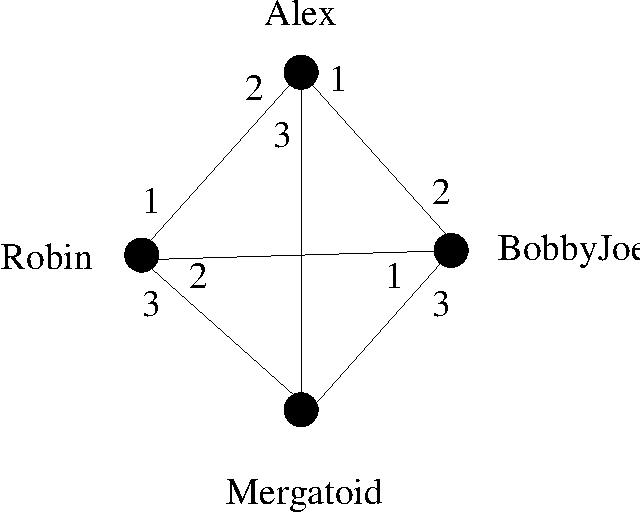
\includegraphics[height=2.3in]{figures/loveTriangle.pdf}
\caption{Some preferences with no stable buddy matching.}
\label{fig:buddy}
\end{figure}
 
Let's see why there is no stable matching: 
\begin{lemma*}
There is no stable buddy matching among the four people in
Figure~\ref{fig:buddy}.
\end{lemma*}
 
\begin{proof}
We'll prove this by contradiction.

Assume, for the purposes of contradiction, that there is a stable
matching.  Then there are two members of the love triangle that are
matched.  Since preferences in the triangle are symmetric, we may assume
in particular, that Robin and Alex are matched.  Then the other pair must
be Bobby-Joe matched with Mergatoid.

But then there is a rogue couple: Alex likes Bobby-Joe best, and Bobby-Joe
prefers Alex to his buddy Mergatoid.  That is, Alex and Bobby-Joe are a
rogue couple, contradicting the assumed stability of the matching.
\end{proof}

So getting a stable \emph{buddy} matching may not only be hard, it may be
impossible.  But when boys are only allowed to marry girls, and vice
versa, then it turns out that a stable matching is not hard to find.

%%insert rest of story from gusfield book pp3--4??

\iffalse

\subsection{Failed attempts}

Let's find a stable matching in one possible situation, and hope to
translate our method to a general algorithm.  The table below shows the
preferences of each girl and boy in decreasing order.

\begin{eqnarray*}
boys & \quad & girls \\
1 : C B E A D & \quad & A : 3 5 2 1 4 \\
2 : A B E C D & \quad & B : 5 2 1 4 3 \\
3 : D C B A E & \quad & C : 4 3 5 1 2 \\
4 : A C D B E & \quad & D : 1 2 3 4 5 \\
5 : A B D E C & \quad & E : 2 3 4 1 5
\end{eqnarray*}

How about we try a ``greedy'' strategy?\footnote{``Greedy'' is not any
moral judgment.  It refers to algorithms that work by always choosing the
next state that makes the largest immediate progress.}  We simply take
each boy in turn and pack him off with his favorite among the girls still
available.  This gives the following assignment.

\begin{eqnarray*}
1 \rightarrow C \\
2 \rightarrow A \\
3 \rightarrow D \\
4 \rightarrow B \\
5 \rightarrow E \\
\end{eqnarray*}

To determine whether this matching is stable, we have to check whether
there are any rogue couples.  Boys 1, 2, and 3 all got their top pick
among the girls; none would even think of running off.  Boy 4 may be a
problem because he likes girl $A$ better than his mate, but she ranks him
dead last.  However, boy 4 also likes girl $C$ better than his mate, and
she rates him above her own mate.  Therefore, boy 4 and girl $C$ form a
rogue couple!  The marriages are not stable.  We could try to make ad hoc
repairs, but we're really trying to develop a general strategy.

Another approach would be to use induction.  Suppose we pair Boy 1 with
his favorite girl, $C$, try to show that neither of these two will be
involved in a rogue couple, and then solve the remaining problem by
induction.  Clearly Boy 1 will never leave his top pick, Girl $C$.  But
the problem with this approach is that we \emph{can't} be sure that Girl
$C$ won't be in a rogue couple.  Girl $C$ might very well dump Boy 1 --
she might even rate him last!

This turns out to be a tricky problem.  The best approach is to use a
mating ritual that is reputed to have been popular in some mythic past.
\fi

\subsection{The Mating Ritual}

The procedure for finding a stable matching involves a \emph{Mating
Ritual} that takes place over several days.  The following events happen
each day:

{\bf Morning: } Each girl stands on her balcony.  Each boy stands under
the balcony of his favorite among the girls on his list, and he serenades
her.  If a boy has no girls left on his list, he stays home and does his
6.042 homework.

{\bf Afternoon: } Each girl who has one or more suitors serenading her,
says to her favorite suitor, ``We might get engaged.  Come back
tomorrow.''  To the others, she says, ``No.  I will never marry you!  Take
a hike!''

\textbf{Evening}: Any boy who is told by a girl to take a hike, crosses that
girl off his list.

\textbf{Termination condition}: When every girl has at most one suitor,
the ritual ends with each girl marrying her suitor, if she has one.

% Show example

There are a number of facts about this Mating Ritual that we would like to
prove:

\begin{itemize}
\item The Ritual has a last day.
\item Everybody ends up married.
\item The resulting marriages are stable.
\end{itemize}

\subsection{A State Machine Model}

Before we can prove anything, we should have clear mathematical
definitions of what we're talking about.  In this section we sketch how to
define a rigorous state machine model of the Marriage Problem.

So let's begin by formally defining the problem.

\begin{definition}
A \term{Marriage Problem} consists of two disjoint sets of the same finite
size, called \boys\ and \girls.  The members of \boys\ are called
\emph{boys}, and members of \girls\ are called \emph{girls}.  For each
boy, $B$, there is a strict total order, $<_B$, on \girls, and for each
girl, $G$, there is a strict total order, $<_G$, on \boys.  If $G_1 <_B
G_2$ we say $B$ \term{prefers} girl $G_2$ to girl $G_1$.  Similarly, if
$B_1 <_G B_2$ we say $G$ \term{prefers} boy $B_2$ to boy $B_1$.

A \emph{marriage assignment} or \term{perfect matching} is a bijection,
$w:\boys \to \girls$.  If $B \in \boys$, then $w(B)$ is called $B$'s
\emph{wife} in the assignment, and if $G \in \girls$, then $w^{-1}(G)$ is
called $G$'s \emph{husband}.  A \term{rogue couple} is a boy, $B$, and a
girl, $G$, such that $B$ prefers $G$ to his wife, and $G$ prefers $B$ to
her husband.  An assignment is \term{stable} if it has no rogue couples.
A \term{solution} to a marriage problem is a stable perfect matching.
\end{definition}

To model the Mating Ritual with a state machine, we make a key
observation: to determine what happens on any day of the Ritual, all we
need to know is which girls are on which boys' lists on the morning of
that day.  So we define a state to be some mathematical data structure
providing this information.  For example, we could define a state to be
the ``still-has-on-his-list'' relation, $R$, between boys and girls, where
$B\,R\,G$ means girl $G$ is still on boy $B$'s list.

We start the Mating Ritual with no girls crossed off.  That is, the start
state is the \emph{complete bipartite} relation in which every boy is
related to every girl.

According to the Mating Ritual, on any given morning, a boy will
\emph{serenade} the girl he most prefers among those he has not as yet
crossed out.  Mathematically, the girl he is serenading is just the
maximum among the girls on $B$'s list, ordered by $<_B$.  (If the list is
empty, he's not serenading anybody.)  A girl's \emph{favorite} is just the
maximum, under her preference ordering, among the boys serenading her.

Continuing in this way, we could mathematically specify a precise Mating
Ritual state machine, but we won't bother.  The intended behavior of the
Mating Ritual is clear enough that we don't gain much by giving a formal
state machine, so we stick to a more memorable description in terms of
boys, girls, and their preferences.  The point is, though, that it's not
hard to define everything using basic mathematical data structures like
sets, functions, and relations, if need be.

\subsection{There is a Marriage Day}

It's easy to see why the Mating Ritual has a terminal day when people
finally get married.  Every day on which the ritual hasn't terminated, at
least one boy crosses a girl off his list.  (If the ritual hasn't
terminated, there must be some girl serenaded by at least two boys, and at
least one of them will have to cross her off his list).  So starting with
$n$ boys and $n$ girls, each of the $n$ boys' lists initially has $n$
girls on it, for a total of $n^2$ list entries.  Since no girl ever gets
added to a list, the total number of entries on the lists decreases every
day that the Ritual continues, and so the Ritual can continue for at most
$n^2$ days.

\subsection{They All Live Happily Every After...}

We still have to prove that the Mating Ritual leaves everyone in a
stable marriage.  To do this, we note one very useful fact about the
Ritual: if a girl has a favorite boy suitor on some morning of the Ritual,
then that favorite suitor will still be serenading her the next morning
---because his list won't have changed.  So she is sure to have today's
favorite boy among her suitors tomorrow.  That means she will be able to
choose a favorite suitor tomorrow who is at least as desirable to her as
today's favorite.  So day by day, her favorite suitor can stay the same or
get better, never worse.  In others words, a girl's favorite is a weakly
increasing variable with respect to her preference order on the boys.

Now we can verify the Mating Ritual using a simple invariant predicate,
$P$, that captures what's going on:
\begin{quotation}
  For every girl, $G$, and every boy, $B$, if $G$ is crossed off $B$'s
  list, then $G$ has a suitor whom she prefers over $B$.
\end{quotation}

Why is $P$ invariant?  Well, we know that $G$'s favorite tomorrow will be
at least as desirable to her as her favorite today, and since her favorite
today is more desirable than $B$, tomorrow's favorite will be too.

Notice that $P$ also holds on the first day, since every girl is on every
list.  So by the Invariant Theorem, we know that $P$ holds on every day
that the Mating Ritual runs.  Knowing the invariant holds when the
Mating Ritual terminates will let us complete the proofs.

\begin{theorem}
Everyone is married by the Mating Ritual.
\end{theorem}

\begin{proof}
  Suppose, for the sake of contradiction, that it is the last day of
  the Mating Ritual and some boy does not get married.  Then he can't
  be serenading anybody, and so his list must be empty.  So by invariant
  $P$, every girl has a favorite boy whom she prefers to that boy.  In
  particular, every girl has a favorite boy whom she marries on the
  last day.  So all the girls are married.  What's more there is no
  bigamy: a boy only serenades one girl, so no two girls have the same
  favorite.

But there are the same number of girls as boys, so all the boys must be
married too.
\end{proof}

\begin{theorem}
The Mating Ritual produces a stable matching.
\end{theorem}

\begin{proof}
Let Brad be some boy and Jen be any girl that he is \emph{not} married to
on the last day of the Mating Ritual.  We claim that Brad and Jen are not
a rogue couple.  Since Brad is an arbitrary boy, it follows that no boy is
part of a rogue couple.  Hence the marriages on the last day are stable.

To prove the claim, we consider two cases:

\emph{Case} 1.  Jen is not on Brad's list.  Then by invariant $P$, we know
that Jen prefers her husband to Brad.  So she's not going to run off with
Brad: the claim holds in this case.

\emph{Case} 2.  Otherwise, Jen is on Brad's list.  But since Brad is not
married to Jen, he must be choosing to serenade his wife instead of Jen,
so he must prefer his wife.  So he's not going to run off with Jen: the
claim also holds in this case.
\end{proof}


\subsection{...Especially the Boys}

Who is favored by the Mating Ritual, the boys or the girls?  The girls
seem to have all the power: they stand on their balconies choosing the
finest among their suitors and spurning the rest.  What's more, we know
their suitors can only change for the better as the Ritual progresses.
Similarly, a boy keeps serenading the girl he most prefers among those on
his list until he must cross her off, at which point he serenades the next
most preferred girl on his list.  So from the boy's point of view, the
girl he is serenading can only change for the worse.  Sounds like a good
deal for the girls.

But it's not!  The fact is that from the beginning, the boys are
serenading their first choice girl, and the desirability of the girl being
serenaded decreases only enough to give the boy his most desirable
possible spouse.  The mating algorithm actually does as well as possible
for all the boys and does the worst possible job for the girls.

To explain all this we need some definitions.  Let's begin by observing
that while the mating algorithm produces one stable matching, there may be
other stable matchings among the same set of boys and girls.  For example,
reversing the roles of boys and girls will often yield a different stable
matching among them.

But some spouses might be out of the question in all possible stable
matchings.  For example, Brad is just not in the realm of possibility for
Jennifer, since if you ever pair them, Brad and Angelina will form a rogue
couple; here's a picture:

\mfigure{!}{1.2in}{figures/exampleOpt}

\begin{definition}
Given any marriage problem, one person is in another person's \emph{realm
of possible spouses} if there is a stable matching in which the two people
are married.  A person's {\em optimal spouse} is their most preferred
person within their realm of possibility.  A person's {\em pessimal
spouse} is their least preferred person in their realm of possibility.
\end{definition}

Everybody has an optimal and a pessimal spouse, since we know there is at
least one stable matching, namely the one produced by the Mating Ritual.
Now here is the shocking truth about the Mating Ritual:

\begin{theorem}\label{boyopt}
The Mating Ritual marries every boy to his optimal spouse.
\end{theorem}

\begin{proof}
Assume for the purpose of contradiction that some boy does not get his
optimal girl.  There must have been a day when he crossed off his optimal
girl ---otherwise he would still be serenading her or some even more
desirable girl.

By the Well Ordering Principle, there must be a \emph{first} day when a
boy, call him ``Keith,'' crosses off his optimal girl, Nicole.

According to the rules of the Ritual, Keith crosses off Nicole because
Nicole has a favorite suitor, Tom, and
\begin{quote}
Nicole prefers Tom to Keith (*)
\end{quote}
(remember, this is a proof by contradiction \texttt{:-)} ).

Now since this is the first day an optimal girl gets crossed off, we know
Tom hasn't crossed off his optimal girl.  So
\begin{quote}
Tom ranks Nicole at least as high as his optimal girl. (**)
\end{quote}
By the definition of an optimal girl, there must be some stable set of
marriages in which Keith gets his optimal girl, Nicole.  But then the
preferences given in ~(*) and~(**) imply that Nicole and Tom are a
rogue couple within this supposedly stable set of marriages (think
about it).  This is a contradiction.
\end{proof}

\begin{theorem}
The Mating Ritual marries every girl to her pessimal spouse.
\end{theorem}

\begin{proof}
Say Nicole and Keith marry each other as a result of the Mating Ritual.
By the previous Theorem~\ref{boyopt}, Nicole is Keith's optimal spouse,
and so in any stable set of marriages,
\begin{quote}
Keith rates Nicole at least as high as his spouse. (+)
\end{quote}

Now suppose for the purpose of contradiction that there is another stable
set of marriages where Nicole does worse than Keith.  That is, Nicole is
married to Tom, and
\begin{quote}
Nicole prefers Keith to Tom (++)
\end{quote}
Then in this stable set of marriages where Nicole is married to Tom,~(+)
and~(++) imply that Nicole and Keith are a rogue couple, contradicting
stability.  We conclude that Nicole cannot do worse than Keith.
\end{proof}

\begin{problems}
\practiceproblems

\pinput{TP_mating_ritual_invariant}

\homeworkproblems

\pinput{PS_stable_matching_no_first_choice}

\pinput{PS_stable_matching_non-optimal}

\pinput{PS_stable_matching_hospitals}

\pinput{PS_stable_matching_unlucky}

\end{problems}


\subsection{Applications}

Not surprisingly, a stable matching procedure is used by at least one
large dating agency.  But although ``boy-girl-marriage'' terminology is
traditional and makes some of the definitions easier to remember (we hope
without offending anyone), solutions to the Stable Marriage Problem are
widely useful.

The Mating Ritual was first announced in a paper by D. Gale and
L.S. Shapley in 1962, but ten years before the Gale-Shapley paper was
appeared, and unbeknownst to them, the Ritual was being used to assign
residents to hospitals by the National Resident Matching Program (NRMP).
The NRMP has, since the turn of the twentieth century, assigned each
year's pool of medical school graduates to hospital residencies (formerly
called ``internships'') with hospitals and graduates playing the roles of
boys and girls.  (In this case there may be multiple boys married to one
girl, but there's an easy way to use the Ritual in this situation.)
Before the Ritual was adopted, there were chronic disruptions and awkward
countermeasures taken to preserve assignments of graduates to residencies.
The Ritual resolved these problems so successfully, that it was used
essentially without change at least through 1989.\footnote{Much more about
the Stable Marriage Problem can be found in the very readable mathematical
monograph by Dan Gusfield and Robert W. Irving,
\href{http://mitpress.mit.edu/catalog/item/default.asp?ttype=2&tid=7676}{The
Stable Marriage Problem: Structure and Algorithms}, MIT Press, Cambridge,
Massachusetts, 1989, 240 pp.}

MIT Math Prof.\ Tom Leighton, who regularly teaches 6.042 and also founded
the internet infrastructure company, Akamai, reports another application.
Akamai uses a variation of the Gale-Shapley procedure to assign web
traffic to servers.  In the early days, Akamai used other combinatorial
optimization algorithms that got to be too slow as the number of servers
and traffic increased.  Akamai switched to Gale-Shapley since it is fast
and can be run in a distributed manner.  In this case, the web traffic
corresponds to the boys and the web servers to the girls.  The servers
have preferences based on latency and packet loss; the traffic has
preferences based on the cost of bandwidth.

\endinput
